% =============================================================================
% APPENDIX BN: REF-LEAD: Lead Management System
% =============================================================================
% Category: REF
% Module: BCM2_SALES_LEAD
% Version: 1.0 (February 2026)
% Status: Final
% Language: English
%
% Comprehensive documentation of the FehrAdvice Lead Management System,
% covering the complete lifecycle from lead creation to closure, including
% the 3-layer ID prevention architecture, data model, workflows, and automation.
%
% =============================================================================

% =============================================================================
% CROSS-REFERENCE STRUCTURE
% =============================================================================
%
% CHAPTER LINKAGE (Required):
% - Primary Chapter: None (Operational Reference)
% - Secondary Chapters: N/A
%
% This appendix provides operational reference for:
%
% DEPENDENCIES (what this appendix REQUIRES):
% - Appendix G: Glossary (standard terms)
%
% DEPENDENTS (what REQUIRES this appendix):
% - Sales Team: Daily lead management operations
% - Claude Code: Automated lead creation workflows
%
% =============================================================================

\begin{tcolorbox}[colback=purple!5!white, colframe=purple!75!black,
    title=Chapter Linkage]

\textbf{Primary Chapter:} Operational Reference (no chapter link)

\textbf{Usage Context:}
\begin{itemize}[nosep]
\item Sales operations and lead management
\item Claude Code automation for /lead-add and /meeting workflows
\item Data integrity maintenance for lead-database.yaml
\end{itemize}

\textbf{Reading Guide:}
\begin{itemize}[nosep]
\item For quick start: See Section~\ref{sec:bn-quickstart}
\item For ID system: See Section~\ref{sec:bn-id-system}
\item For troubleshooting: See Section~\ref{sec:bn-troubleshooting}
\end{itemize}

\end{tcolorbox}

\chapter{REF-LEAD: Lead Management System}
\label{app:lead-system}


\begin{tcolorbox}[colback=blue!5!white, colframe=blue!75!black,
    title=Quick Reference: Appendix UNMAPPED_BN]

\textbf{Appendix:} BN (REF-LEAD)

\textbf{Core Question:} How does the FehrAdvice Lead Management System work from creation to closure?

\textbf{Key Concepts:}
\begin{itemize}[nosep]
\item Lead Lifecycle: SUSPECT $\to$ PROSPECT $\to$ QUALIFIED $\to$ PROPOSAL $\to$ NEGOTIATION $\to$ CLOSED
\item 3-Layer ID System: Atomic Script + Workflow Docs + Auto-Fix Hook
\item Data Model: lead-database.yaml with customer/person integrations
\end{itemize}

\textbf{Cross-References:} Appendix G (Glossary), data/sales/LEAD-ID-SYSTEM.md
\end{tcolorbox}


\begin{abstract}
This appendix documents the complete FehrAdvice Lead Management System, providing operational guidance for the sales pipeline from lead identification through closure. It covers the 6-stage lifecycle model, the 3-layer ID prevention architecture that ensures data integrity, the YAML-based data model with cross-references to customer and person profiles, and the automated workflows including /lead-add and /meeting slash commands. The system integrates with Claude Code for automation while maintaining human oversight for strategic decisions.
\end{abstract}


\begin{tcolorbox}[
    colback=orange!5!white,
    colframe=orange!75!black,
    title={\textbf{Appendix Scope: Ziel / In-Scope / Out-of-Scope / Constraints}},
    fonttitle=\bfseries
]

\textbf{Ziel (Objective):}
\begin{itemize}[nosep]
    \item Document the complete Lead Management System for FehrAdvice sales operations
\end{itemize}

\textbf{In-Scope:}
\begin{itemize}[nosep]
    \item Lead Lifecycle (6 stages from SUSPECT to CLOSED)
    \item LEAD-ID System (3-layer architecture for duplicate prevention)
    \item Data Model (YAML structure, fields, relationships)
    \item Workflows (/lead-add, /meeting, stage transitions)
    \item Automation (scripts, pre-commit hooks)
    \item Integration with customer/person profiles
\end{itemize}

\textbf{Out-of-Scope (delegiert an andere Appendices):}
\begin{itemize}[nosep]
    \item Customer profiling methodology $\rightarrow$ Context Vector Architecture (CVA)
    \item Behavioral scoring models $\rightarrow$ Appendix TKT (METHOD-TOOLKIT)
    \item Pipeline forecasting $\rightarrow$ /forecast skill documentation
\end{itemize}

\textbf{Constraints (Anwendungsgrenzen):}
\begin{itemize}[nosep]
    \item System designed for FehrAdvice-specific workflows
    \item Requires Claude Code environment for automation
    \item YAML-based storage (not a traditional CRM database)
\end{itemize}

\textbf{Lieferobjekte (Deliverables):}
\begin{itemize}[nosep]
    \item Lead Lifecycle State Machine (Figure~\ref{fig:bn-lifecycle})
    \item 3-Layer ID Architecture (Figure~\ref{fig:bn-id-architecture})
    \item Data Model Schema (Table~\ref{tab:bn-schema})
    \item Workflow Checklists (Tables~\ref{tab:bn-lead-add}, \ref{tab:bn-stage-transition})
\end{itemize}

\end{tcolorbox}


% =============================================================================
% PART 2: CORE CONTENT
% =============================================================================

%%%%%%%%%%%%%%%%%%%%%%%%%%%%%%%%%%%%%%%%%%%%%%%%%%%%%%%%%%%%%%%%%%%%%%%%%%%%%%%
\section{The Fundamental Question}
\label{sec:bn-fundamental}
%%%%%%%%%%%%%%%%%%%%%%%%%%%%%%%%%%%%%%%%%%%%%%%%%%%%%%%%%%%%%%%%%%%%%%%%%%%%%%%

\subsection{Why This Matters}

Effective lead management is critical for consulting firms where:
\begin{itemize}
    \item Sales cycles are long (months to years)
    \item Relationships are paramount (trust-based selling)
    \item Pipeline visibility drives resource allocation
    \item Historical data enables continuous improvement
\end{itemize}

Traditional CRM systems are often overkill for boutique consulting firms, while spreadsheets lack structure and auditability. The FehrAdvice Lead Management System provides a middle ground: structured YAML data with Git versioning, automated workflows via Claude Code, and human-readable documentation.

\subsection{The Core Problem}

\begin{tcolorbox}[colback=red!5!white, colframe=red!75!black,
    title=The Fundamental Question]
\textbf{How can we manage the complete lead lifecycle with data integrity, automation, and full auditability while maintaining human control over strategic decisions?}
\end{tcolorbox}


%%%%%%%%%%%%%%%%%%%%%%%%%%%%%%%%%%%%%%%%%%%%%%%%%%%%%%%%%%%%%%%%%%%%%%%%%%%%%%%
\section{Core Theory: Sales Pipeline Management}
\label{sec:bn-theory}
%%%%%%%%%%%%%%%%%%%%%%%%%%%%%%%%%%%%%%%%%%%%%%%%%%%%%%%%%%%%%%%%%%%%%%%%%%%%%%%

The Lead Management System is built on established sales pipeline theory, adapted for consulting services.

\subsection{Pipeline Theory Foundations}

The system implements three core theoretical principles:

\begin{enumerate}
    \item \textbf{Stage-Gate Model:} Leads progress through defined stages with explicit entry/exit criteria, enabling systematic qualification and forecasting.
    \item \textbf{Single Source of Truth (SSOT):} All lead data resides in one authoritative location (\texttt{lead-database.yaml}), eliminating synchronization issues.
    \item \textbf{Defense in Depth:} Multiple layers of validation (script, workflow, hook) ensure data integrity even when individual layers fail.
\end{enumerate}

\subsection{Design Principles}

\begin{itemize}
    \item \textbf{Atomic Operations:} ID generation is atomic (read-increment-write in single operation) to prevent race conditions.
    \item \textbf{Immutable History:} Stage transitions are append-only; history is never modified.
    \item \textbf{Bidirectional References:} Cross-references between leads, customers, and persons enable navigation in both directions.
    \item \textbf{Human-Readable Storage:} YAML format allows manual inspection and Git-based version control.
\end{itemize}


%%%%%%%%%%%%%%%%%%%%%%%%%%%%%%%%%%%%%%%%%%%%%%%%%%%%%%%%%%%%%%%%%%%%%%%%%%%%%%%
\section{Axioms and Rules}
\label{sec:bn-axioms}
%%%%%%%%%%%%%%%%%%%%%%%%%%%%%%%%%%%%%%%%%%%%%%%%%%%%%%%%%%%%%%%%%%%%%%%%%%%%%%%

The Lead Management System operates under the following axioms and rules.

\begin{tcolorbox}[colback=gray!5!white, colframe=gray!75!black,
    title=Axiom LM-A1: Single Source of Truth]
\textbf{Statement:} The \texttt{metadata.next\_lead\_id} field in \texttt{lead-database.yaml} is the sole authoritative source for the next available LEAD-ID.

\textbf{Interpretation:} No other location (memory, cache, external system) may be used to determine the next ID.

\textbf{Implication:} All ID generation must read from and write to this field atomically.
\end{tcolorbox}

\begin{tcolorbox}[colback=gray!5!white, colframe=gray!75!black,
    title=Axiom LM-A2: Forward-Only Progression]
\textbf{Statement:} For any lead $L$, if $\text{stage}(L, t_1) = S_i$ and $\text{stage}(L, t_2) = S_j$ where $t_2 > t_1$, then $j \geq i$ (except for CLOSED\_LOST which can be reached from any stage).

\textbf{Interpretation:} Leads cannot regress to earlier stages; they can only advance or be closed as lost.

\textbf{Implication:} Prevents artificial pipeline manipulation and ensures forecast accuracy.
\end{tcolorbox}

\begin{tcolorbox}[colback=gray!5!white, colframe=gray!75!black,
    title=Axiom LM-A3: Referential Integrity]
\textbf{Statement:} For every reference $R$ in a lead entry, the referenced entity must exist: $\forall R \in \text{Lead}: \exists E \text{ where } R \to E$.

\textbf{Interpretation:} Customer profiles, person profiles, and meeting references must resolve to existing files.

\textbf{Implication:} The creation cascade (Customer $\to$ Person $\to$ Lead) must be followed in order.
\end{tcolorbox}

\begin{tcolorbox}[colback=gray!5!white, colframe=gray!75!black,
    title=Axiom LM-A4: Audit Trail Completeness]
\textbf{Statement:} Every state change must be recorded: $\forall \Delta S: \exists H \in \text{stage\_history}$ documenting date, owner, and reason.

\textbf{Interpretation:} No stage transition occurs without documentation.

\textbf{Implication:} Enables pipeline velocity analysis and accountability.
\end{tcolorbox}


%%%%%%%%%%%%%%%%%%%%%%%%%%%%%%%%%%%%%%%%%%%%%%%%%%%%%%%%%%%%%%%%%%%%%%%%%%%%%%%
\section{Lead Lifecycle}
\label{sec:bn-lifecycle}
%%%%%%%%%%%%%%%%%%%%%%%%%%%%%%%%%%%%%%%%%%%%%%%%%%%%%%%%%%%%%%%%%%%%%%%%%%%%%%%

The Lead Lifecycle consists of 6 stages, each with defined entry criteria, exit criteria, and actions.

\subsection{Stage Definitions}

\begin{figure}[htbp]
\centering
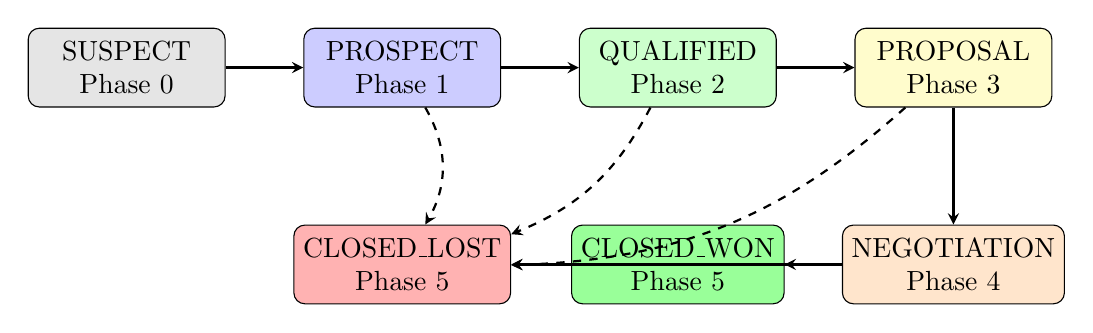
\begin{tikzpicture}[
    stage/.style={rectangle, draw, rounded corners, minimum width=2.5cm, minimum height=1cm, align=center},
    arrow/.style={->, thick, >=stealth}
]
% Stages
\node[stage, fill=gray!20] (suspect) at (0,0) {SUSPECT\\Phase 0};
\node[stage, fill=blue!20] (prospect) at (3.5,0) {PROSPECT\\Phase 1};
\node[stage, fill=green!20] (qualified) at (7,0) {QUALIFIED\\Phase 2};
\node[stage, fill=yellow!20] (proposal) at (10.5,0) {PROPOSAL\\Phase 3};
\node[stage, fill=orange!20] (negotiation) at (10.5,-2.5) {NEGOTIATION\\Phase 4};
\node[stage, fill=green!40] (won) at (7,-2.5) {CLOSED\_WON\\Phase 5};
\node[stage, fill=red!30] (lost) at (3.5,-2.5) {CLOSED\_LOST\\Phase 5};

% Arrows
\draw[arrow] (suspect) -- (prospect);
\draw[arrow] (prospect) -- (qualified);
\draw[arrow] (qualified) -- (proposal);
\draw[arrow] (proposal) -- (negotiation);
\draw[arrow] (negotiation) -- (won);
\draw[arrow] (negotiation) -- (lost);

% Skip arrows (dashed)
\draw[arrow, dashed] (prospect) to[bend left=30] (lost);
\draw[arrow, dashed] (qualified) to[bend left=20] (lost);
\draw[arrow, dashed] (proposal) to[bend left=20] (lost);

\end{tikzpicture}
\caption{Lead Lifecycle State Machine}
\label{fig:bn-lifecycle}
\end{figure}

\begin{table}[htbp]
\centering
\caption{Lead Stages: Definitions and Criteria}
\label{tab:bn-stages}
\renewcommand{\arraystretch}{1.4}
\begin{tabular}{@{}p{2.5cm}p{3cm}p{3cm}p{4cm}@{}}
\toprule
\textbf{Stage} & \textbf{Entry Criteria} & \textbf{Exit Criteria} & \textbf{Key Actions} \\
\midrule
\textbf{SUSPECT} (Phase 0) &
Potential fit identified &
First contact made &
Research, outreach planning \\

\textbf{PROSPECT} (Phase 1) &
Contact established &
Need confirmed, budget discussed &
Discovery meeting, needs analysis \\

\textbf{QUALIFIED} (Phase 2) &
BANT confirmed\footnotemark &
Proposal requested &
Solution design, stakeholder mapping \\

\textbf{PROPOSAL} (Phase 3) &
Proposal submitted &
Decision pending &
Proposal presentation, Q\&A \\

\textbf{NEGOTIATION} (Phase 4) &
Terms being discussed &
Agreement reached or rejected &
Contract negotiation, terms alignment \\

\textbf{CLOSED\_WON} (Phase 5) &
Contract signed &
-- &
Handoff to delivery, kickoff \\

\textbf{CLOSED\_LOST} (Phase 5) &
Opportunity rejected &
-- &
Loss analysis, relationship maintenance \\
\bottomrule
\end{tabular}
\end{table}
\footnotetext{BANT = Budget, Authority, Need, Timeline}

\subsection{Stage Transition Rules}

\begin{tcolorbox}[colback=gray!5!white, colframe=gray!75!black,
    title=Rule LM-1: Forward Progression]
\textbf{Statement:} Leads can only progress forward through stages (SUSPECT $\to$ PROSPECT $\to$ ...).

\textbf{Exception:} Any stage can transition directly to CLOSED\_LOST.

\textbf{Rationale:} Prevents artificial pipeline inflation and ensures accurate forecasting.
\end{tcolorbox}

\begin{tcolorbox}[colback=gray!5!white, colframe=gray!75!black,
    title=Rule LM-2: Stage History]
\textbf{Statement:} Every stage transition must be recorded in \texttt{stage\_history[]} with date, owner, and reason.

\textbf{Rationale:} Enables pipeline velocity analysis and identifies bottlenecks.
\end{tcolorbox}

\begin{tcolorbox}[colback=gray!5!white, colframe=gray!75!black,
    title=Rule LM-3: Mandatory Fields per Stage]
\textbf{Statement:} Each stage has required fields that must be populated before transition.

\begin{itemize}[nosep]
\item PROSPECT: \texttt{contacts[]} must have at least one entry
\item QUALIFIED: \texttt{opportunities[]} must have value estimate
\item PROPOSAL: \texttt{opportunities[].proposal\_date} must be set
\item CLOSED\_WON: \texttt{opportunities[].value\_eur} must be confirmed
\end{itemize}
\end{tcolorbox}


%%%%%%%%%%%%%%%%%%%%%%%%%%%%%%%%%%%%%%%%%%%%%%%%%%%%%%%%%%%%%%%%%%%%%%%%%%%%%%%
\section{LEAD-ID System: 3-Layer Architecture}
\label{sec:bn-id-system}
%%%%%%%%%%%%%%%%%%%%%%%%%%%%%%%%%%%%%%%%%%%%%%%%%%%%%%%%%%%%%%%%%%%%%%%%%%%%%%%

The LEAD-ID System prevents duplicate IDs through a defense-in-depth architecture with three layers.

\begin{figure}[htbp]
\centering
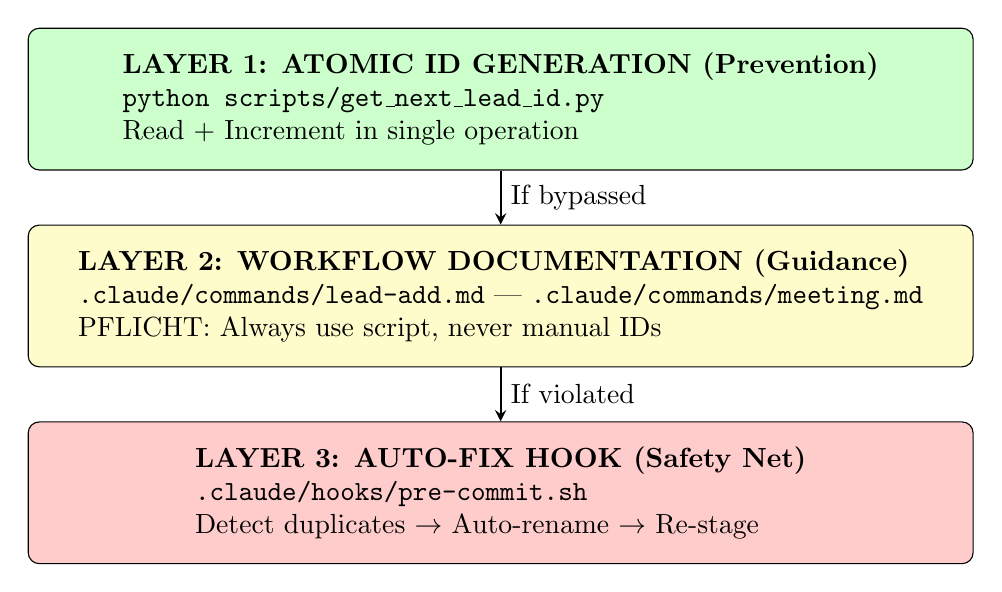
\begin{tikzpicture}[
    layer/.style={rectangle, draw, rounded corners, minimum width=12cm, minimum height=1.8cm, align=left},
    arrow/.style={->, thick, >=stealth}
]

\node[layer, fill=green!20] (layer1) at (0,4) {
    \textbf{LAYER 1: ATOMIC ID GENERATION (Prevention)}\\
    \texttt{python scripts/get\_next\_lead\_id.py}\\
    Read + Increment in single operation
};

\node[layer, fill=yellow!20] (layer2) at (0,1.5) {
    \textbf{LAYER 2: WORKFLOW DOCUMENTATION (Guidance)}\\
    \texttt{.claude/commands/lead-add.md} | \texttt{.claude/commands/meeting.md}\\
    PFLICHT: Always use script, never manual IDs
};

\node[layer, fill=red!20] (layer3) at (0,-1) {
    \textbf{LAYER 3: AUTO-FIX HOOK (Safety Net)}\\
    \texttt{.claude/hooks/pre-commit.sh}\\
    Detect duplicates $\to$ Auto-rename $\to$ Re-stage
};

\draw[arrow] (layer1) -- node[right] {If bypassed} (layer2);
\draw[arrow] (layer2) -- node[right] {If violated} (layer3);

\end{tikzpicture}
\caption{3-Layer LEAD-ID Architecture}
\label{fig:bn-id-architecture}
\end{figure}

\subsection{Layer 1: Atomic ID Generation}

The \texttt{get\_next\_lead\_id.py} script provides atomic ID generation:

\begin{verbatim}
# Standard usage: Get ID and increment
python scripts/get_next_lead_id.py
# Output: LEAD-061
# Effect: next_lead_id incremented to 62

# Peek mode: Check without incrementing
python scripts/get_next_lead_id.py --peek
# Output: LEAD-061
# Effect: None (read-only)

# Validation: Check database consistency
python scripts/get_next_lead_id.py --validate
# Output: Consistency status + statistics
\end{verbatim}

\textbf{Single Source of Truth (SSOT):} The \texttt{metadata.next\_lead\_id} field in \texttt{lead-database.yaml} is the authoritative source for the next available ID.

\subsection{Layer 2: Workflow Documentation}

All workflows that create leads must call the script:

\begin{table}[htbp]
\centering
\caption{Workflow Integration Points}
\label{tab:bn-workflow-integration}
\renewcommand{\arraystretch}{1.3}
\begin{tabular}{@{}lll@{}}
\toprule
\textbf{Workflow} & \textbf{File} & \textbf{Integration Step} \\
\midrule
/lead-add & \texttt{.claude/commands/lead-add.md} & Step 1: Call script before YAML creation \\
/meeting & \texttt{.claude/commands/meeting.md} & Step 0: Call script before cascade \\
Manual & N/A & VERBOTEN (forbidden) \\
\bottomrule
\end{tabular}
\end{table}

\subsection{Layer 3: Auto-Fix Hook}

The pre-commit hook provides automatic duplicate resolution:

\begin{enumerate}
\item \textbf{Detection:} Scan for duplicate LEAD-IDs in staged changes
\item \textbf{Resolution:} Keep first occurrence, rename subsequent via script
\item \textbf{Annotation:} Add comment \texttt{\# Auto-fixed from LEAD-XXX}
\item \textbf{Re-stage:} Automatically stage corrected file
\item \textbf{Correction:} Update \texttt{next\_lead\_id} if inconsistent
\end{enumerate}

\begin{tcolorbox}[colback=green!5!white, colframe=green!75!black,
    title=Auto-Fix Example]
\begin{verbatim}
$ git commit -m "Add two new leads"

=== EBF PreCommit: Checking LEAD-ID Uniqueness ===
⚠️  LEAD-ID CONFLICT: Duplicate IDs found - AUTO-FIXING...
   Keeping LEAD-048 at line 245 (original)
   🔄 Renaming LEAD-048 → LEAD-061 at line 312 (auto-fix)
   ✅ Fixed and re-staged lead-database.yaml

=== All compliance checks passed ===
[main abc1234] Add two new leads
\end{verbatim}
\end{tcolorbox}


%%%%%%%%%%%%%%%%%%%%%%%%%%%%%%%%%%%%%%%%%%%%%%%%%%%%%%%%%%%%%%%%%%%%%%%%%%%%%%%
\section{Data Model}
\label{sec:bn-data-model}
%%%%%%%%%%%%%%%%%%%%%%%%%%%%%%%%%%%%%%%%%%%%%%%%%%%%%%%%%%%%%%%%%%%%%%%%%%%%%%%

\subsection{Lead Entry Schema}

\begin{table}[htbp]
\centering
\caption{Lead Entry Schema (lead-database.yaml)}
\label{tab:bn-schema}
\renewcommand{\arraystretch}{1.2}
\begin{tabular}{@{}p{3.5cm}p{2cm}p{6cm}@{}}
\toprule
\textbf{Field} & \textbf{Type} & \textbf{Description} \\
\midrule
\multicolumn{3}{l}{\textit{Identification}} \\
\texttt{id} & string & LEAD-NNN (from script) \\
\texttt{company.name} & string & Full company name \\
\texttt{company.short\_name} & string & Abbreviated name \\
\texttt{company.ref} & path & Reference to customer profile \\
\midrule
\multicolumn{3}{l}{\textit{Classification}} \\
\texttt{industry} & enum & Branche (finance, packaging, etc.) \\
\texttt{segment} & enum & enterprise / mid\_market / smb / government \\
\texttt{country} & string & ISO country code (CH, AT, DE) \\
\midrule
\multicolumn{3}{l}{\textit{Pipeline Status}} \\
\texttt{stage} & enum & Current stage (SUSPECT...CLOSED) \\
\texttt{stage\_history[]} & array & All stage transitions with dates \\
\texttt{owner} & string & Responsible partner initials \\
\midrule
\multicolumn{3}{l}{\textit{Contacts}} \\
\texttt{contacts[]} & array & Contact persons \\
\texttt{contacts[].name} & string & Full name \\
\texttt{contacts[].profile\_ref} & path & Reference to person profile \\
\texttt{contacts[].is\_decision\_maker} & bool & Decision authority \\
\midrule
\multicolumn{3}{l}{\textit{Opportunities}} \\
\texttt{opportunities[]} & array & Business opportunities \\
\texttt{opportunities[].name} & string & Opportunity description \\
\texttt{opportunities[].value\_eur} & number & Estimated value \\
\texttt{opportunities[].probability} & number & Win probability (0-1) \\
\midrule
\multicolumn{3}{l}{\textit{Source \& Tracking}} \\
\texttt{source.channel} & enum & REFERRAL / INBOUND / OUTBOUND / RESEARCH \\
\texttt{source.referrer} & string & Referrer name (if REFERRAL) \\
\texttt{created} & date & Creation date \\
\texttt{updated} & date & Last modification date \\
\bottomrule
\end{tabular}
\end{table}

\subsection{Cross-Reference Architecture}

The Lead Management System maintains bidirectional references with customer and person profiles:

\begin{figure}[htbp]
\centering
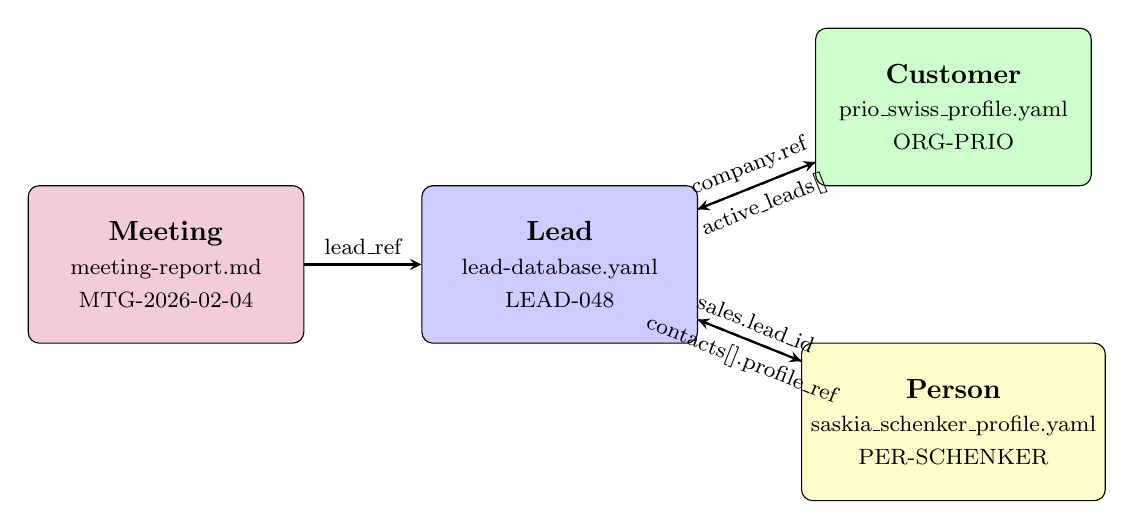
\begin{tikzpicture}[
    entity/.style={rectangle, draw, rounded corners, minimum width=3.5cm, minimum height=2cm, align=center},
    arrow/.style={->, thick, >=stealth}
]

\node[entity, fill=blue!20] (lead) at (0,0) {
    \textbf{Lead}\\
    \footnotesize lead-database.yaml\\
    \footnotesize LEAD-048
};

\node[entity, fill=green!20] (customer) at (5,2) {
    \textbf{Customer}\\
    \footnotesize prio\_swiss\_profile.yaml\\
    \footnotesize ORG-PRIO
};

\node[entity, fill=yellow!20] (person) at (5,-2) {
    \textbf{Person}\\
    \footnotesize saskia\_schenker\_profile.yaml\\
    \footnotesize PER-SCHENKER
};

\node[entity, fill=purple!20] (meeting) at (-5,0) {
    \textbf{Meeting}\\
    \footnotesize meeting-report.md\\
    \footnotesize MTG-2026-02-04
};

% Forward references (solid)
\draw[arrow] (lead) -- node[above, sloped, font=\footnotesize] {company.ref} (customer);
\draw[arrow] (lead) -- node[below, sloped, font=\footnotesize] {contacts[].profile\_ref} (person);
\draw[arrow] (meeting) -- node[above, font=\footnotesize] {lead\_ref} (lead);

% Back references (dashed)
\draw[arrow, dashed] (customer) -- node[below, sloped, font=\footnotesize] {active\_leads[]} (lead);
\draw[arrow, dashed] (person) -- node[above, sloped, font=\footnotesize] {sales.lead\_id} (lead);

\end{tikzpicture}
\caption{Cross-Reference Architecture}
\label{fig:bn-cross-ref}
\end{figure}

\begin{table}[htbp]
\centering
\caption{Reference Directions}
\label{tab:bn-references}
\renewcommand{\arraystretch}{1.3}
\begin{tabular}{@{}llll@{}}
\toprule
\textbf{From} & \textbf{To} & \textbf{Field} & \textbf{Example} \\
\midrule
Lead & Customer & \texttt{company.ref} & \texttt{customers/prio-swiss} \\
Lead & Person & \texttt{contacts[].profile\_ref} & \texttt{saskia\_schenker\_profile.yaml} \\
Customer & Lead & \texttt{active\_leads[]} & \texttt{["LEAD-048"]} \\
Person & Lead & \texttt{sales.lead\_id} & \texttt{LEAD-048} \\
Meeting & Lead & \texttt{lead\_ref} & \texttt{LEAD-048} \\
\bottomrule
\end{tabular}
\end{table}


%%%%%%%%%%%%%%%%%%%%%%%%%%%%%%%%%%%%%%%%%%%%%%%%%%%%%%%%%%%%%%%%%%%%%%%%%%%%%%%
\section{Workflows}
\label{sec:bn-workflows}
%%%%%%%%%%%%%%%%%%%%%%%%%%%%%%%%%%%%%%%%%%%%%%%%%%%%%%%%%%%%%%%%%%%%%%%%%%%%%%%

\subsection{Creating a New Lead (/lead-add)}
\label{sec:bn-lead-add}

\begin{table}[htbp]
\centering
\caption{/lead-add Workflow Checklist}
\label{tab:bn-lead-add}
\renewcommand{\arraystretch}{1.3}
\begin{tabular}{@{}clll@{}}
\toprule
\textbf{Step} & \textbf{Action} & \textbf{Command/Tool} & \textbf{Output} \\
\midrule
1 & Get Lead ID & \texttt{python scripts/get\_next\_lead\_id.py} & LEAD-NNN \\
2 & Create customer profile (if new) & Write YAML & \texttt{customers/\{org\}/} \\
3 & Create person profile (if new) & Write YAML & \texttt{\{person\}\_profile.yaml} \\
4 & Add lead entry & Edit lead-database.yaml & New lead record \\
5 & Update back-references & Edit customer/person profiles & \texttt{active\_leads[]}, etc. \\
6 & Commit & git commit & Version recorded \\
\bottomrule
\end{tabular}
\end{table}

\subsection{Meeting with Lead Creation (/meeting)}

When a meeting results in a new lead, the workflow follows this cascade:

\begin{verbatim}
Step 0: LEAD-ID HOLEN (PFLICHT!)
        python scripts/get_next_lead_id.py → "LEAD-061"

Step 1: KUNDE erstellen (falls neu)
        data/customers/{org}/{org}_profile.yaml

Step 2: PERSON erstellen (falls neu)
        data/customers/{org}/{person}_profile.yaml

Step 3: LEAD erstellen (mit ID aus Schritt 0)
        data/sales/lead-database.yaml

Step 4: RÜCK-REFERENZEN aktualisieren
        - customer.active_leads[] += "LEAD-061"
        - person.sales.lead_id = "LEAD-061"

Step 5: OUTPUTS generieren
        - Meeting Report
        - Begleitschreiben (if applicable)
\end{verbatim}

\subsection{Stage Transitions (/lead-update)}

\begin{table}[htbp]
\centering
\caption{Stage Transition Checklist}
\label{tab:bn-stage-transition}
\renewcommand{\arraystretch}{1.3}
\begin{tabular}{@{}llp{6cm}@{}}
\toprule
\textbf{Transition} & \textbf{Required Fields} & \textbf{Validation} \\
\midrule
SUSPECT $\to$ PROSPECT & \texttt{contacts[]} & At least one contact with name \\
PROSPECT $\to$ QUALIFIED & \texttt{opportunities[].value\_eur} & Value estimate required \\
QUALIFIED $\to$ PROPOSAL & \texttt{opportunities[].proposal\_date} & Proposal submission date \\
PROPOSAL $\to$ NEGOTIATION & -- & Verbal or written interest \\
NEGOTIATION $\to$ CLOSED\_WON & \texttt{opportunities[].closed\_date} & Signed contract \\
Any $\to$ CLOSED\_LOST & \texttt{loss\_reason} & Reason for loss documented \\
\bottomrule
\end{tabular}
\end{table}


%%%%%%%%%%%%%%%%%%%%%%%%%%%%%%%%%%%%%%%%%%%%%%%%%%%%%%%%%%%%%%%%%%%%%%%%%%%%%%%
\section{Worked Example}
\label{sec:bn-example}
%%%%%%%%%%%%%%%%%%%%%%%%%%%%%%%%%%%%%%%%%%%%%%%%%%%%%%%%%%%%%%%%%%%%%%%%%%%%%%%

\subsection{Example: prio.swiss Lead Creation}

\paragraph{Setup.} On 2026-02-04, Gerhard Fehr meets Saskia Schenker (Director of prio.swiss) at Jacks Brasserie. This is a first meeting with a potential new client.

\paragraph{Application.}

\textbf{Step 0: Get Lead ID}
\begin{verbatim}
$ python scripts/get_next_lead_id.py
✅ next_lead_id: 48 → 49
LEAD-048
\end{verbatim}

\textbf{Step 1: Create Customer Profile}
\begin{verbatim}
# data/customers/prio-swiss/prio_swiss_profile.yaml
id: "ORG-PRIO"
slug: "prio-swiss"
name: "prio.swiss"
classification:
  industry: "professional_services"
  industry_subcategory: "insurance_association"
\end{verbatim}

\textbf{Step 2: Create Person Profile}
\begin{verbatim}
# data/customers/prio-swiss/saskia_schenker_profile.yaml
id: "PER-SCHENKER"
personal:
  first_name: "Saskia"
  last_name: "Schenker"
  title: "Dr."
professional:
  position: "Direktorin"
  is_decision_maker: true
\end{verbatim}

\textbf{Step 3: Create Lead Entry}
\begin{verbatim}
# data/sales/lead-database.yaml (new entry)
- id: LEAD-048
  company:
    name: "prio.swiss"
    ref: "customers/prio-swiss"
  industry: "professional_services"
  stage: PROSPECT
  stage_history:
    - stage: PROSPECT
      date: "2026-02-04"
      owner: GF
      reason: "First meeting at Jacks Brasserie"
  contacts:
    - name: "Dr. Saskia Schenker"
      profile_ref: "saskia_schenker_profile.yaml"
      is_decision_maker: true
  source:
    channel: OUTBOUND
    first_touch_date: "2026-02-04"
\end{verbatim}

\textbf{Step 4: Update Back-References}
\begin{verbatim}
# prio_swiss_profile.yaml
sales:
  active_leads: ["LEAD-048"]

# saskia_schenker_profile.yaml
sales:
  lead_id: "LEAD-048"
\end{verbatim}

\paragraph{Result.} Lead LEAD-048 is created with full bidirectional references. The atomic ID system ensures no duplicates. The pre-commit hook will validate on commit.

\paragraph{Discussion.} This example shows the complete cascade from meeting to lead creation. The 3-layer ID system ensures that even if Claude bypasses Step 0, the pre-commit hook will catch and fix any duplicates.


%%%%%%%%%%%%%%%%%%%%%%%%%%%%%%%%%%%%%%%%%%%%%%%%%%%%%%%%%%%%%%%%%%%%%%%%%%%%%%%
\section{Troubleshooting}
\label{sec:bn-troubleshooting}
%%%%%%%%%%%%%%%%%%%%%%%%%%%%%%%%%%%%%%%%%%%%%%%%%%%%%%%%%%%%%%%%%%%%%%%%%%%%%%%

\begin{table}[htbp]
\centering
\caption{Common Issues and Solutions}
\label{tab:bn-troubleshooting}
\renewcommand{\arraystretch}{1.4}
\begin{tabular}{@{}p{4cm}p{4cm}p{5cm}@{}}
\toprule
\textbf{Problem} & \textbf{Cause} & \textbf{Solution} \\
\midrule
Duplicate LEAD-ID in commit & Manual ID assignment & Let auto-fix hook handle it, or manually run script \\

\texttt{next\_lead\_id} too low & Direct YAML edit & Run \texttt{--validate} and manually correct \\

Script not found & Wrong directory & Run from repository root \\

Pre-commit hook not running & Hook not installed & Check \texttt{.claude/hooks/pre-commit.sh} \\

References broken & Missing profile file & Create customer/person profile first \\
\bottomrule
\end{tabular}
\end{table}

\subsection{Validation Commands}

\begin{verbatim}
# Check database consistency
python scripts/get_next_lead_id.py --validate

# Preview next ID without incrementing
python scripts/get_next_lead_id.py --peek

# Manual duplicate check
grep -E "^  - id: LEAD-[0-9]+" data/sales/lead-database.yaml | sort | uniq -d
\end{verbatim}


%%%%%%%%%%%%%%%%%%%%%%%%%%%%%%%%%%%%%%%%%%%%%%%%%%%%%%%%%%%%%%%%%%%%%%%%%%%%%%%
\section{Quick Start Guide}
\label{sec:bn-quickstart}
%%%%%%%%%%%%%%%%%%%%%%%%%%%%%%%%%%%%%%%%%%%%%%%%%%%%%%%%%%%%%%%%%%%%%%%%%%%%%%%

\begin{tcolorbox}[colback=green!5!white, colframe=green!75!black,
    title=Quick Start: Creating a Lead]

\textbf{Option A: Via /lead-add (recommended)}
\begin{verbatim}
/lead-add "Company Name" industry
\end{verbatim}

\textbf{Option B: Via /meeting (after meeting)}
\begin{verbatim}
/meeting new
# Follow prompts, select "Lead eröffnen" when asked
\end{verbatim}

\textbf{Option C: Manual (advanced)}
\begin{enumerate}[nosep]
\item \texttt{python scripts/get\_next\_lead\_id.py} $\to$ get LEAD-NNN
\item Create customer profile (if new)
\item Create person profile (if new)
\item Add entry to lead-database.yaml with LEAD-NNN
\item Update back-references
\item \texttt{git add \&\& git commit}
\end{enumerate}

\textbf{NEVER:}
\begin{itemize}[nosep]
\item[$\times$] Manually assign a LEAD-ID
\item[$\times$] Copy an existing ID
\item[$\times$] Guess the next available ID
\end{itemize}

\end{tcolorbox}


% =============================================================================
% PART 4: BACK MATTER
% =============================================================================

%%%%%%%%%%%%%%%%%%%%%%%%%%%%%%%%%%%%%%%%%%%%%%%%%%%%%%%%%%%%%%%%%%%%%%%%%%%%%%%
\section{Summary}
\label{sec:bn-summary}
%%%%%%%%%%%%%%%%%%%%%%%%%%%%%%%%%%%%%%%%%%%%%%%%%%%%%%%%%%%%%%%%%%%%%%%%%%%%%%%

\begin{tcolorbox}[colback=green!10!white, colframe=green!75!black,
    title=\textbf{Appendix UNMAPPED_BN: Summary}]

\textbf{Core Question:} How does the FehrAdvice Lead Management System work?

\textbf{Main Contribution:}
\begin{itemize}[nosep]
    \item 6-stage lifecycle model (SUSPECT $\to$ CLOSED)
    \item 3-layer ID prevention architecture
    \item YAML-based data model with cross-references
    \item Automated workflows via Claude Code
\end{itemize}

\textbf{Key Outputs:}
\begin{itemize}[nosep]
    \item Atomic ID script: \texttt{scripts/get\_next\_lead\_id.py}
    \item Auto-fix hook: \texttt{.claude/hooks/pre-commit.sh}
    \item Workflow docs: \texttt{.claude/commands/lead-add.md}, \texttt{meeting.md}
\end{itemize}

\textbf{Integration:} The Lead Management System integrates with customer profiles (CVA), person profiles, and meeting documentation to provide a complete sales pipeline view.

\end{tcolorbox}


%%%%%%%%%%%%%%%%%%%%%%%%%%%%%%%%%%%%%%%%%%%%%%%%%%%%%%%%%%%%%%%%%%%%%%%%%%%%%%%
\section{Glossary of Terms}
\label{sec:bn-glossary}
%%%%%%%%%%%%%%%%%%%%%%%%%%%%%%%%%%%%%%%%%%%%%%%%%%%%%%%%%%%%%%%%%%%%%%%%%%%%%%%

\begin{tcolorbox}[colback=blue!5!white, colframe=blue!75!black]
\textbf{Central Reference:} For complete symbol definitions, see
\textbf{Appendix G} (\textit{Glossary and Notation}).

This section lists only terms introduced in this appendix.
\end{tcolorbox}

\vspace{0.5em}

\begin{table}[htbp]
\centering
\caption{Terms Introduced in Appendix UNMAPPED_BN}
\label{tab:bn-glossary}
\renewcommand{\arraystretch}{1.3}
\begin{tabular}{@{}p{3cm}p{9cm}@{}}
\toprule
\textbf{Term} & \textbf{Definition} \\
\midrule
LEAD-ID & Unique identifier for a lead in format LEAD-NNN (e.g., LEAD-048) \\
Stage & Current position in the sales pipeline (SUSPECT, PROSPECT, etc.) \\
BANT & Budget, Authority, Need, Timeline - qualification criteria \\
Atomic ID Generation & Script that reads and increments ID in a single operation \\
Auto-Fix Hook & Pre-commit hook that automatically resolves duplicate IDs \\
Back-Reference & Reverse link from customer/person profile to lead \\
\bottomrule
\end{tabular}
\end{table}


%%%%%%%%%%%%%%%%%%%%%%%%%%%%%%%%%%%%%%%%%%%%%%%%%%%%%%%%%%%%%%%%%%%%%%%%%%%%%%%
\section{Critical Foundations and Objections}
\label{sec:bn-foundations}
%%%%%%%%%%%%%%%%%%%%%%%%%%%%%%%%%%%%%%%%%%%%%%%%%%%%%%%%%%%%%%%%%%%%%%%%%%%%%%%

\subsection{Objection 1: YAML is Not a Database}

\begin{tcolorbox}[colback=red!5!white, colframe=red!50!black,
    title=Objection: YAML lacks database features]
YAML files lack transactions, indexes, and query capabilities that traditional databases provide. This could lead to data corruption or performance issues at scale.
\end{tcolorbox}

\textbf{Response:} For a boutique consulting firm with 50-200 leads, YAML provides sufficient performance while offering advantages: human readability, Git versioning (full audit trail), and no database administration overhead. The atomic script and pre-commit hooks provide transaction-like guarantees for the most critical operation (ID generation). If scale becomes an issue ($>$1000 leads), migration to SQLite or PostgreSQL with YAML export is straightforward.

\subsection{Objection 2: Manual Processes are Error-Prone}

\begin{tcolorbox}[colback=red!5!white, colframe=red!50!black,
    title=Objection: Human error in data entry]
Despite automation, users may still make errors in data entry, especially for non-automated fields like opportunity values or contact information.
\end{tcolorbox}

\textbf{Response:} The 3-layer architecture specifically addresses the highest-risk error (duplicate IDs). For other fields, the system relies on:
\begin{itemize}[nosep]
    \item Schema validation (stage must be valid enum)
    \item Required field checks per stage transition
    \item Git history for error detection and rollback
    \item Human review in the /meeting and /lead-add workflows
\end{itemize}

\subsection{Objection 3: Dependency on Claude Code}

\begin{tcolorbox}[colback=red!5!white, colframe=red!50!black,
    title=Objection: System requires AI assistant]
The system relies on Claude Code for automation. What happens when Claude is unavailable or makes errors?
\end{tcolorbox}

\textbf{Response:} The system is designed to work without Claude:
\begin{itemize}[nosep]
    \item Manual workflow documented in Appendix UNMAPPED_BN and LEAD-ID-SYSTEM.md
    \item Script can be run directly: \texttt{python scripts/get\_next\_lead\_id.py}
    \item Pre-commit hook runs independently of Claude
    \item All data is human-readable YAML
\end{itemize}
Claude accelerates workflows but is not a single point of failure.


%%%%%%%%%%%%%%%%%%%%%%%%%%%%%%%%%%%%%%%%%%%%%%%%%%%%%%%%%%%%%%%%%%%%%%%%%%%%%%%
\section{CRM Feature Comparison}
\label{sec:bn-crm-comparison}
%%%%%%%%%%%%%%%%%%%%%%%%%%%%%%%%%%%%%%%%%%%%%%%%%%%%%%%%%%%%%%%%%%%%%%%%%%%%%%%

This section compares the FehrAdvice Lead Management System against standard CRM features found in systems like Salesforce, HubSpot, or Pipedrive.

\subsection{Feature Matrix}

\begin{table}[htbp]
\centering
\caption{CRM Feature Comparison Matrix}
\label{tab:bn-crm-features}
\renewcommand{\arraystretch}{1.2}
\begin{tabular}{@{}p{4cm}ccp{5cm}@{}}
\toprule
\textbf{Feature} & \textbf{Status} & \textbf{Effort} & \textbf{Notes} \\
\midrule
\multicolumn{4}{l}{\textit{Lead Lifecycle Management}} \\
\midrule
Pipeline Stages & \checkmark & -- & 11 stages implemented \\
Stage History & \checkmark & -- & Full audit trail \\
Lead Scoring & \checkmark & -- & fit\_score + engagement\_score \\
Owner Assignment & \checkmark & -- & Team registry with OWN-xxx \\
Deadline Management & \checkmark & -- & Auto-deadlines per stage \\
\midrule
\multicolumn{4}{l}{\textit{Data Integrity}} \\
\midrule
Unique ID Generation & \checkmark & -- & 3-layer architecture \\
Duplicate Prevention & \checkmark & -- & Auto-fix hook \\
Cross-References & \checkmark & -- & Customer $\leftrightarrow$ Person $\leftrightarrow$ Lead \\
\midrule
\multicolumn{4}{l}{\textit{Notifications \& Automation}} \\
\midrule
Email Notifications & \checkmark & -- & On lead creation \\
Deadline Reminders & \checkmark & -- & Configurable \\
Stage Change Alerts & $\circ$ & 1h & Config exists, not active \\
\midrule
\multicolumn{4}{l}{\textit{Activity \& Communication (GAP)}} \\
\midrule
Activity Log & $\times$ & \textbf{2h} & Add \texttt{activities:[]} to lead schema \\
Task Management & $\times$ & \textbf{2h} & Add \texttt{tasks:[]} with due dates \\
Communication History & $\times$ & \textbf{2h} & Track emails, calls per lead \\
\midrule
\multicolumn{4}{l}{\textit{Analytics (GAP)}} \\
\midrule
Pipeline Velocity & $\times$ & \textbf{4h} & Calculate from stage\_history \\
Win/Loss Analysis & $\times$ & \textbf{3h} & Structured close reasons \\
Forecast Report & $\times$ & \textbf{4h} & Probability $\times$ Value \\
Source ROI & $\times$ & 8h & Conversion by source channel \\
\midrule
\multicolumn{4}{l}{\textit{Advanced (Requires Integration)}} \\
\midrule
Email Integration & $\times$ & 40h+ & Needs external API \\
Calendar Sync & $\times$ & 40h+ & Needs external API \\
Marketing Automation & $\times$ & 80h+ & Needs external platform \\
Mobile App & $\times$ & 200h+ & Out of scope for CLI \\
\bottomrule
\end{tabular}
\end{table}

\textbf{Legend:} \checkmark = Implemented, $\circ$ = Partially implemented, $\times$ = Not implemented

\subsection{Immediately Implementable Features}

The following features can be added within hours using the existing YAML/Git architecture:

\subsubsection{1. Activity Log (2 hours)}

Track all interactions per lead:

\begin{lstlisting}[language=yaml,basicstyle=\ttfamily\small]
activities:
  - id: ACT-001
    type: call          # call, email, meeting, note
    date: "2026-02-04"
    owner: GF
    summary: "Discovery call with Saskia Schenker"
    duration_minutes: 30
    outcome: "Interest confirmed, send proposal"
    next_action: "Send proposal by Feb 10"
\end{lstlisting}

\textbf{Implementation:}
\begin{enumerate}[nosep]
    \item Add \texttt{activities:[]} to lead schema
    \item Create \texttt{/activity-add} slash command
    \item Update \texttt{/lead-card} to show recent activities
\end{enumerate}

\subsubsection{2. Task Management (2 hours)}

Assign follow-up tasks with due dates:

\begin{lstlisting}[language=yaml,basicstyle=\ttfamily\small]
tasks:
  - id: TASK-001
    title: "Send proposal to prio.swiss"
    due_date: "2026-02-10"
    owner: GF
    priority: high       # high, medium, low
    status: open         # open, completed, cancelled
    linked_activity: ACT-001
    created: "2026-02-04"
    completed: null
\end{lstlisting}

\textbf{Implementation:}
\begin{enumerate}[nosep]
    \item Add \texttt{tasks:[]} to lead schema
    \item Create \texttt{/task-add}, \texttt{/task-complete} commands
    \item Add task overview to \texttt{/pipeline-summary}
\end{enumerate}

\subsubsection{3. Win/Loss Analysis (3 hours)}

Structured learning from closed deals:

\begin{lstlisting}[language=yaml,basicstyle=\ttfamily\small]
close_analysis:
  outcome: won           # won, lost
  date: "2026-03-15"

  # For WON deals
  success_factors:
    - "Strong champion (Saskia Schenker)"
    - "Clear budget allocation"
    - "Timing aligned with strategic initiative"

  # For LOST deals
  loss_reason: competitor  # budget, timing, competitor,
                           # no_decision, internal, other
  competitor_name: "McKinsey"
  loss_details: "Client preferred larger brand"
  could_have_won: "Earlier engagement, executive sponsor"

  # Always
  lessons_learned: |
    prio.swiss valued scientific approach but needed
    more case studies from similar organizations.
\end{lstlisting}

\textbf{Implementation:}
\begin{enumerate}[nosep]
    \item Add \texttt{close\_analysis} to lead schema
    \item Update \texttt{/lead-update} for WON/LOST stages
    \item Create \texttt{/win-loss} report command
\end{enumerate}

\subsubsection{4. Pipeline Velocity (4 hours)}

Calculate time spent in each stage:

\begin{lstlisting}[language=yaml,basicstyle=\ttfamily\small]
# Calculated from stage_history automatically
velocity_metrics:
  days_in_suspect: 5
  days_in_prospect: 12
  days_in_qualified: 8
  days_in_proposal: 14
  days_in_negotiation: 7
  total_cycle_time: 46

  # Benchmarks (from won deals)
  vs_average: "+8 days"    # Slower than average
  bottleneck: "proposal"   # Longest stage
\end{lstlisting}

\textbf{Implementation:}
\begin{enumerate}[nosep]
    \item Create \texttt{scripts/calculate\_velocity.py}
    \item Add velocity metrics to \texttt{/pipeline-report}
    \item Generate benchmark from historical data
\end{enumerate}

\subsection{Implementation Priority}

\begin{tcolorbox}[colback=green!5!white, colframe=green!50!black,
    title=Recommended Implementation Order]
\begin{enumerate}
    \item \textbf{Activity Log} (2h) -- Immediate value for tracking touchpoints
    \item \textbf{Task Management} (2h) -- Ensures follow-up discipline
    \item \textbf{Win/Loss Analysis} (3h) -- Learning loop for sales improvement
    \item \textbf{Pipeline Velocity} (4h) -- Identifies process bottlenecks
    \item \textbf{Forecast Report} (4h) -- Revenue planning capability
\end{enumerate}

\textbf{Total: 15 hours} for core CRM parity
\end{tcolorbox}


%%%%%%%%%%%%%%%%%%%%%%%%%%%%%%%%%%%%%%%%%%%%%%%%%%%%%%%%%%%%%%%%%%%%%%%%%%%%%%%
\section{Open Issues and Research Agenda}
\label{sec:bn-open}
%%%%%%%%%%%%%%%%%%%%%%%%%%%%%%%%%%%%%%%%%%%%%%%%%%%%%%%%%%%%%%%%%%%%%%%%%%%%%%%

\begin{table}[htbp]
\centering
\caption{Research Roadmap for Lead Management System}
\label{tab:bn-roadmap}
\renewcommand{\arraystretch}{1.3}
\begin{tabular}{@{}clcl@{}}
\toprule
\textbf{\#} & \textbf{Issue} & \textbf{Priority} & \textbf{Status} \\
\midrule
1 & Pipeline velocity analytics & MEDIUM & Planned \\
2 & Automated stage transition suggestions & LOW & Research \\
3 & Win/loss pattern analysis & MEDIUM & Planned \\
4 & Integration with calendar for touchpoint tracking & LOW & Backlog \\
\bottomrule
\end{tabular}
\end{table}


%%%%%%%%%%%%%%%%%%%%%%%%%%%%%%%%%%%%%%%%%%%%%%%%%%%%%%%%%%%%%%%%%%%%%%%%%%%%%%%
\section{References}
\label{sec:bn-references}
%%%%%%%%%%%%%%%%%%%%%%%%%%%%%%%%%%%%%%%%%%%%%%%%%%%%%%%%%%%%%%%%%%%%%%%%%%%%%%%

\begin{tcolorbox}[colback=blue!5!white, colframe=blue!75!black]
\textbf{Master Bibliography:} For complete reference details, see
\texttt{bcm\_master.bib} in the repository.

This appendix is primarily operational documentation and does not reference academic literature.
\end{tcolorbox}

\subsection{Internal Documentation}

\begin{itemize}[nosep]
    \item \texttt{data/sales/LEAD-ID-SYSTEM.md} -- Detailed ID system documentation
    \item \texttt{.claude/commands/lead-add.md} -- Lead creation workflow
    \item \texttt{.claude/commands/meeting.md} -- Meeting workflow with lead integration
    \item \texttt{scripts/get\_next\_lead\_id.py} -- Atomic ID generation script
\end{itemize}

\nocite{bcm_master}

%%%%%%%%%%%%%%%%%%%%%%%%%%%%%%%%%%%%%%%%%%%%%%%%%%%%%%%%%%%%%%%%%%%%%%%%%%%%%%%
% CROSS-REFERENCE FOOTER
%%%%%%%%%%%%%%%%%%%%%%%%%%%%%%%%%%%%%%%%%%%%%%%%%%%%%%%%%%%%%%%%%%%%%%%%%%%%%%%

\vspace{1em}
\hrule
\vspace{0.5em}

\noindent\textit{Cross-references:}
Appendix G (Central Glossary),
Context Vector Architecture (CVA),
Appendix TKT (METHOD-TOOLKIT).

\noindent\textit{Master Bibliography:} \texttt{bcm\_master.bib}

% =============================================================================
% END OF APPENDIX BN
% =============================================================================
